\section{Introduzione}
\begin{frame}{Contesto}

L’inquinamento atmosferico è uno dei principali problemi che interessano le aree urbanizzate.
\vspace{0.3cm}
\begin{itemize}
 \item Può portare a problemi di salute causati dall’esposizione a lungo termine a sostanze nocive (PM, \ce{NO2}, \ce{CO2}, \ce{O3})\vspace{0.3cm}
 \item Il monitoraggio è essenziale per la tutela della salute pubblica\vspace{0.1cm}
 \begin{enumerate}
 \item Con reti regionali di rilevamento fisse, gestite da ARPA (DLgs. n.155 del 13/08/2010)\vspace{0.1cm}
 \item Con nuove reti di sensori \textit{low cost} ad alta portabilità per l'acquisizione di misure aggiuntive, anche a minor precisione (es. \textbf{AirQino})
\end{enumerate}
\end{itemize}

\end{frame}

\begin{frame}{La piattaforma AirQino (1/3)}
\begin{columns}


\begin{column}{0.4\textwidth}
\begin{center}
\includegraphics[width=.7\textwidth]{images/airqino_stazione}

\begin{itemize}
  \item Monitoraggio ambientale ad alta precisione
  \item Configurabile ed estendibile
\end{itemize}

\end{center}
\end{column}

\begin{column}{0.6\textwidth}

\begin{center}
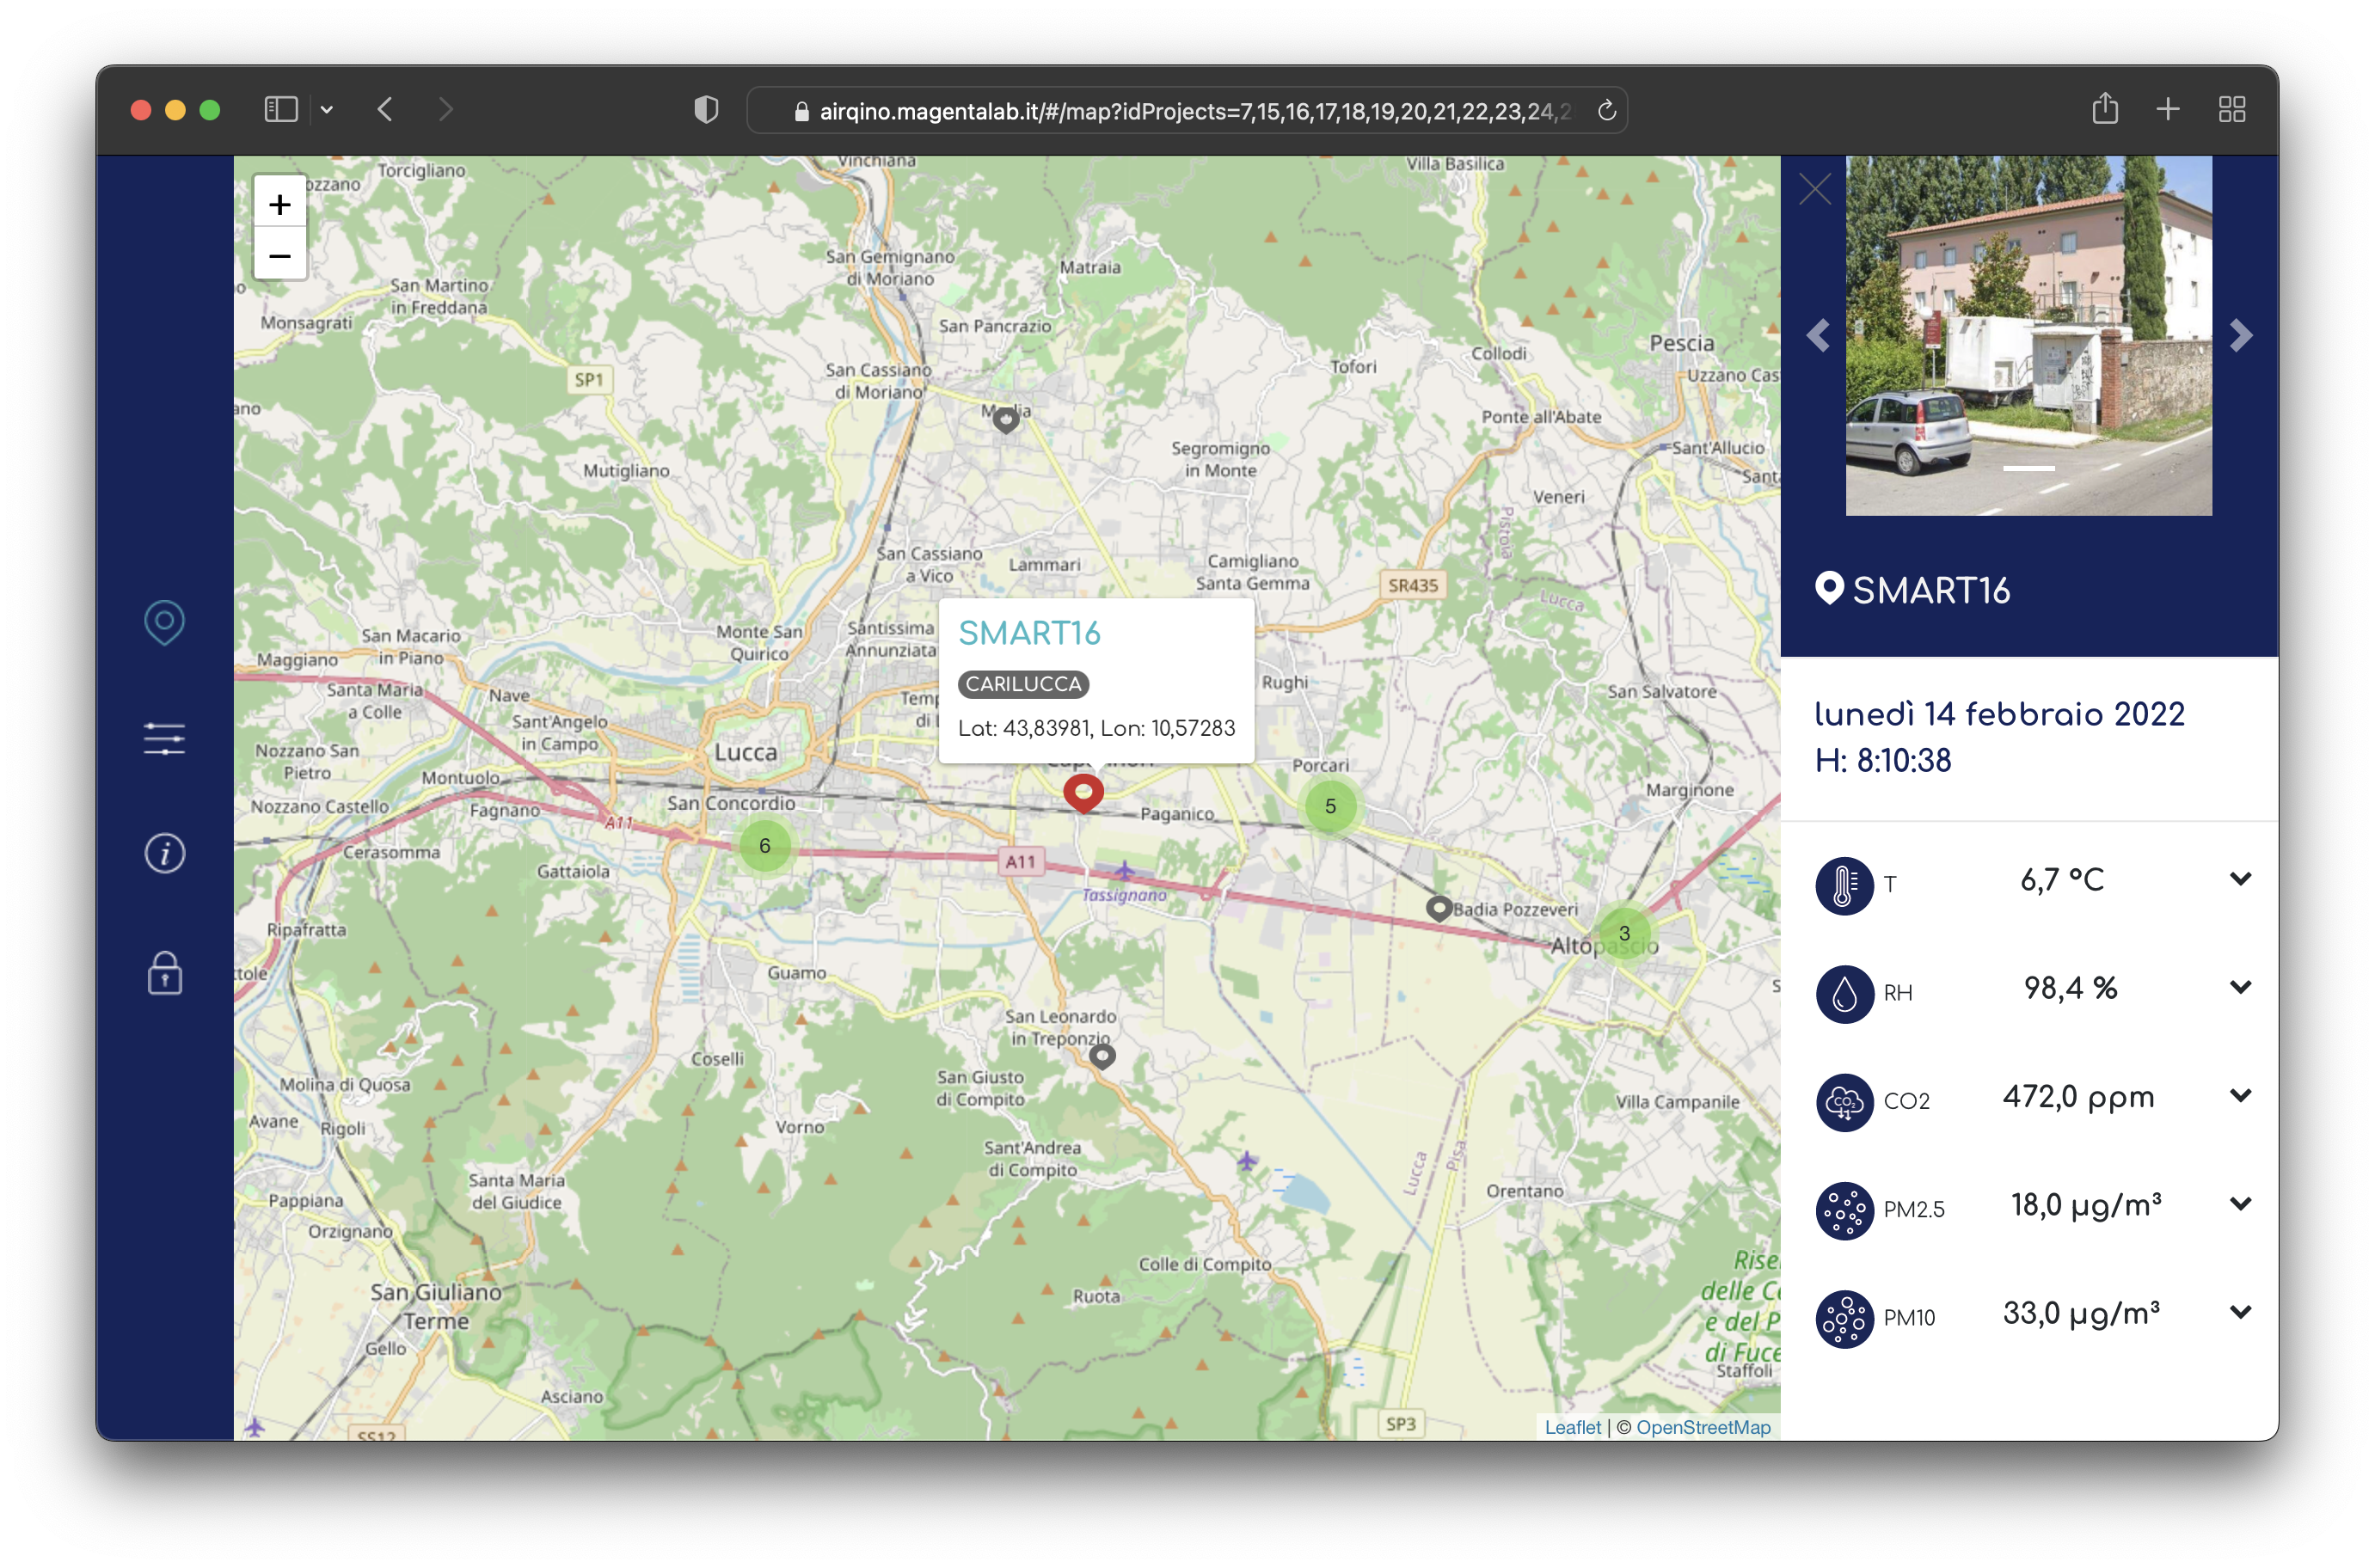
\includegraphics[width=\textwidth]{images/airqino_web}
\alert{https://airqino.magentalab.it}
\end{center}

\end{column}

\end{columns}
\end{frame}

\begin{frame}[t]{La piattaforma AirQino (2/3)}
\begin{center}

\begin{figure}[H]
\centering
\captionsetup{justification=centering}
\includegraphics[width=.8\textwidth]{images/airqino_arch.png}
\caption{Architettura della piattaforma}
\end{figure}

\end{center}
\end{frame}

\begin{frame}[t]{La piattaforma AirQino (3/3)}
\begin{columns}

\begin{column}{0.5\textwidth}
\begin{center}

\begin{block}{MiCS-2714 per \ce{NO2}}
\begin{figure}[H]
    \centering
    \subfloat[\centering Sensore]{{\includegraphics[width=2.4cm]{images/mics1-removebg-preview} }}
    \subfloat[\centering Circuito]{{\includegraphics[width=2.4cm]{images/mics2-removebg-preview} }}
\end{figure}
\vspace{0.1cm}
\begin{itemize}
  \item Di tipo MOS
  \item Basato su ossidoriduzione
  \item Uscita in \textit{counts}
\end{itemize}
\vspace{0.2cm}

\end{block}

\end{center}
\end{column}

\begin{column}{0.5\textwidth}
\begin{center}
\begin{block}{SDS011 per \ce{PM_{2.5}} e \ce{PM_{10}}}
\begin{figure}[H]
    \centering
    \subfloat[\centering Sensore]{{\includegraphics[width=2cm]{images/sds1} }}
    \subfloat[\centering Componenti]{{\includegraphics[width=2.7cm]{images/sds2_rmbg} }}
\end{figure}
\vspace{0.1cm}
\begin{itemize}
  \item Basato su principio di diffusione ottica
  \item Uscita in $\mathrm{\si{\micro}g/m^3}$
  \item Più costoso
\end{itemize}
\vspace{0.2cm}

\end{block}
\end{center}
\end{column}

\end{columns}
\end{frame}

\begin{frame}{Obiettivi}
\begin{itemize}
  \item Sviluppi tecnologici alla piattaforma
  \begin{enumerate}
    \item Miglioramento dell'\textbf{affidabilità} dei dati provenienti dai sensori
    \item Riduzione dei \textbf{tempi di risposta} dal database
  \end{enumerate}\vspace{0.2cm}
  \item Studio e confronto tra diverse tecniche volte a migliorare l’accuratezza del processo di \textbf{calibrazione} dei sensori (sia \ce{NO2} che PM)\vspace{0.2cm}
  \item Sviluppo di un’\textbf{interfaccia web} per facilitare la calibrazione \textit{massiva} di centraline
\end{itemize}
\end{frame}


\section{Sviluppi tecnologici}
\begin{frame}{Replica del database (1/2)}
\end{frame}

\begin{frame}{Replica del database (2/2)}
\end{frame}

\begin{frame}{Ottimizzazione di query temporali (1/2)}
\end{frame}

\begin{frame}{Ottimizzazione di query temporali (2/2)}
\end{frame}

%\section{Calibrazione}
%
%
%\section{Interfaccia}
%
%
%\section{Conclusione}

